\documentclass[../main.tex]{subfiles}
\graphicspath{{\subfix{../images/}}}
\begin{document}

  \textcolor{red}{\textbf{TO-DO}
  \begin{itemize}
    \item Breve introdução ao que será dito no referencial teórico
  \end{itemize}
  }

  \subsection{O robô quadrúpede}
  \textcolor{red}{\textbf{TO-DO}
  \begin{itemize}
    \item Breve introdução ao tópico
  \end{itemize}
  }

  \subsubsection{Apresentação e conceito geral}
  O robô quadrúpede é um sistema robótico móvel que se locomove com a ajuda de pernas. Robôs móveis podem ser divididos em três grupos, relacionados aos seus sistemas de locomoção: robôs com rodas, com esteiras e com pernas. Quando comparado aos dois primeiros, o último grupo apresenta diversas particularidades que os confere muitas vantagens quanto a mobilidade, robustez a diferentes terrenos e superação de obstáculos \textbf{\textcolor{red}{[Fonte: Development of quadruped walking robots: A review]}}. Robôs com rodas e esteiras apresentam boa performance em terrenos planos e conseguem navegar de forma autônoma pelo espaço, desde que haja um caminho contínuo entre os pontos de origem e destino. Robôs com pernas, por outro lado, são capazes de escolher os melhores pontos de suporte no terreno para apoiar seus pés, o que permite uma navegação em caminhos discretos (com obstáculos de grande inclinação e variação de altura) \textbf{\textcolor{red}{[Fonte: Design and driving model for the quadruped robot: An elucidating draft]}}. Essa capacidade de se adaptar de terrenos desnivelados amplia bastante a lista de aplicações às quais esse tipo de sistema pode ser designado: industriais, militares, missões de inspeção, resgate, entre várias outras. Por outro lado, essas vantagens vêm as custa de uma maior complexidade de controle e menor estabilidade. Isso influencia no custo final do sistema, o que pode ser um impeditivo para sua aplicabilidade prática. 

  Robôs com pernas também apresentam diversas diferenças entre si, majoritariamente ligadas à quantidade de pernas que possuem. Entre eles, destacam-se os bípedes, os quadrúpedes e os hexápodes (que podem ser considerados robôs com múltiplas pernas, abrangendo todos com mais de quatro pernas). A quantidade de pernas de um robô está diretamente relacionada a sua estabilidade, capacidade de locomoção e eficiência. Os bípedes possuem baixa estabilidade, visto que se apoiam em apenas uma perna para poder andar e, portanto, necessitam de sistemas de controle complexos para poder de mover. Em contrapartida, os com múltiplas pernas possuem maior estabilidade, afinal conseguem manter pelo menos três (muitas vezes até quatro) pontos de apoio enquanto realizam um passo. Contudo, cada perna apresenta um adicional de juntas e atuadores no sistema, diminuindo a eficiência do sistema como um todo. Os quadrúpedes conseguem unir vantagens dos dois anteriores, ao apresentar um balanço entre estabilidade e eficiência. Eles possuem uma estabilidade passiva, quando estáticos, pois se apoiam em quatro pontos. Além disso, também são capazes de navegar de forma estável em baixas velocidade, movendo uma perna por vez, enquanto as outras três permanecem no solo, o que elimina a redundância e complexidade dos robôs com múltiplas pernas e aumenta sua eficiência \textbf{\textcolor{red}{[Fonte: Design and driving model for the quadruped robot: An elucidating draft]}}.

  \subsubsection{Estrutura e design}
  Por conta das vantagens que apresentam, os robôs quadrúpedes se tornaram um grande foco de pesquisa nos últimos anos. Muitos tipos diferente de designs já foram testados, variando o tipo de perna, modelo de estrutura e número de graus de liberdade (degree of freedom (DOF)) por perna. Alguns designs de quadrúpedes com diferentes tipos de perna e modelos de estrutura podem ser vistos na figura \ref{fig:structure_design}.

  \begin{figure}[h]
    \centering
    \caption{Titulo da Figura}
    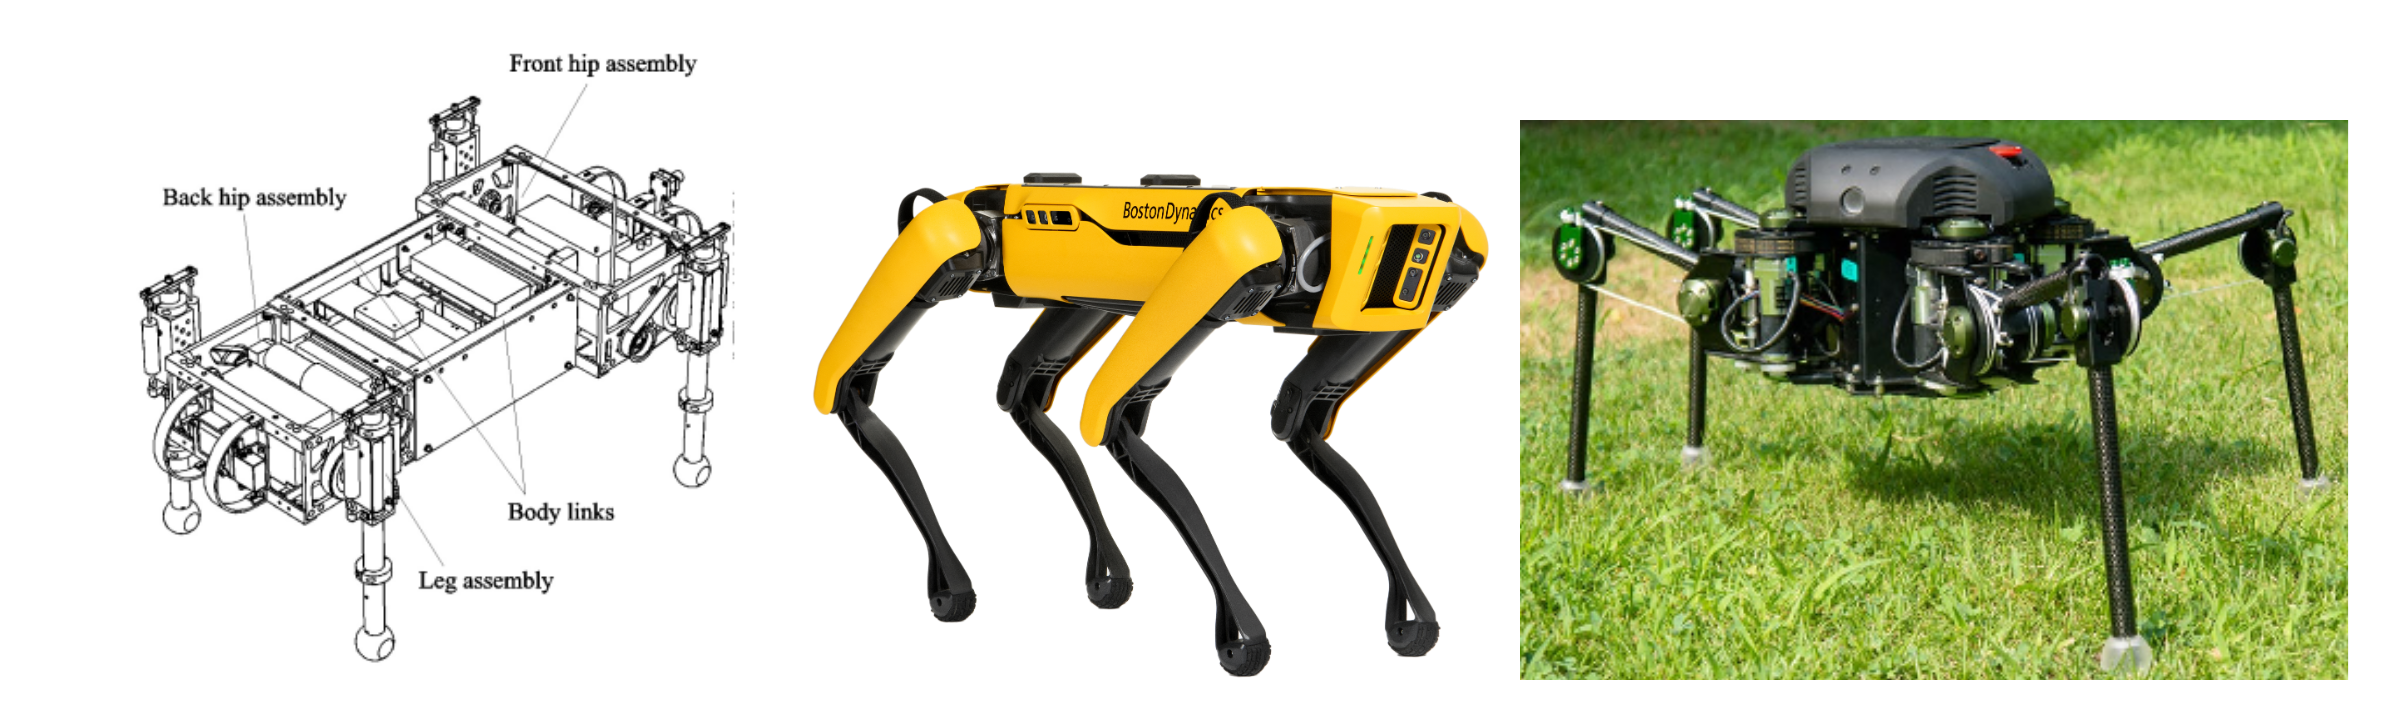
\includegraphics[width=0.8\textwidth]{structure_design.png}
    
    Fonte: XXX
    SCOUT-II / SPOT / TITAN-XIII
    \label{fig:structure_design}
  \end{figure}

  O SCOUT-II, assim como outros robôs que foram alvo de pesquisa na década de 80 por Raibert \textbf{\textcolor{red}{[Legged Robots That Balance]}}, utilizam pernas prismáticas, ou lineares. Isto é, a perna possui apenas uma junta rotativa que a conecta ao corpo e uma junta prismática responsável por aumentar ou diminuir seu comprimento \textbf{\textcolor{red}{[Analysis and research of quadruped robot's legs: A comprehensive review]}}. Essa junta prismática pode ser ativa ou passiva. Juntas ativas podem utilizar pistões ou mecanismos parafusados. Já os de junta passiva, como o SCOUT-II, possuem uma mola com amortecedor, possibilitando a locomoção do robô com base em um movimento oscilatório \textbf{\textcolor{red}{[Quadruped Robot Running With a Bounding Gait ]}}.

  O modelo de estrutura do TITAN-XIII é chamado de sprawling type, que pode ser traduzido para tipo amplo, devido a grande amplitude de abertura das pernas. Já o modelo do Spot, da Boston Dynamics, pode ser chamado de mammal type ou tipo mamífero, por ser inspirado da postura de mamíferos quadrúpedes como cachorros e cavalos. Ambos possuem pernas articuladas com juntas rotativas, podendo variar a quantidade de juntas por perna, a depender do robô. Kitano et al., em \textbf{\textcolor{red}{[TITAN-XIII: sprawling-type quadruped robot with ability of fast and energy-efficient walking]}}, cita algumas vantagens de cada um desses dois modelos de estrutura. O modelo mamífero é capaz de alcançar maiores velocidades, por possuir duas juntas no plano sagital. Além disso, ele também é mais eficiente, pois seus atuadores utilizam menos torque para sustentar o robô, devido à sua estrutura mais compacta, que diminui o braço de alavança sobre o qual a força peso do robô atua. Isso também lhes permite navegar em ambientes estreitos, onde um robô do tipo sprawling teria dificuldades de acessar. Este último, por sua vez, possui uma estrutura que o permite abaixar seu centro de gravidade, dando-lhe mais estabilidade de movimentação e causando menos danos ao robô em caso de quedas, o que é uma vantagem de segurança e confiabilidade. Sua estrutura larga também o permite alcançar pontos de apoio no solo mais distantes do corpo, aumentando seu polígono de suporte. Esse é o polígono paralelo ao solo, cujos vértices são os pés de apoio do robô e sobre o qual o centro de gravidade do sistema deve estar, a fim de garantir estabilidade de movimento. Uma outra vantagem de mobilidade desse tipo de quadrúpede é poder utilizar seu corpo como uma quinta perna, em algumas ocasiões.

  O modelo de estrutura de robô abordado neste trabalho será do tipo mamífero. Entre os robôs quadrúpedes que utilizam esse modelo, eles também se diferenciam quanto ao número de DOF por perna, tipos de atuadores nas juntas e configuração das pernas. Quanto à configuração das pernas, existem quatro tipos, ilustrados na figura abaixo.

  \begin{figure}[h]
    \centering
    \caption{Titulo da Figura}
    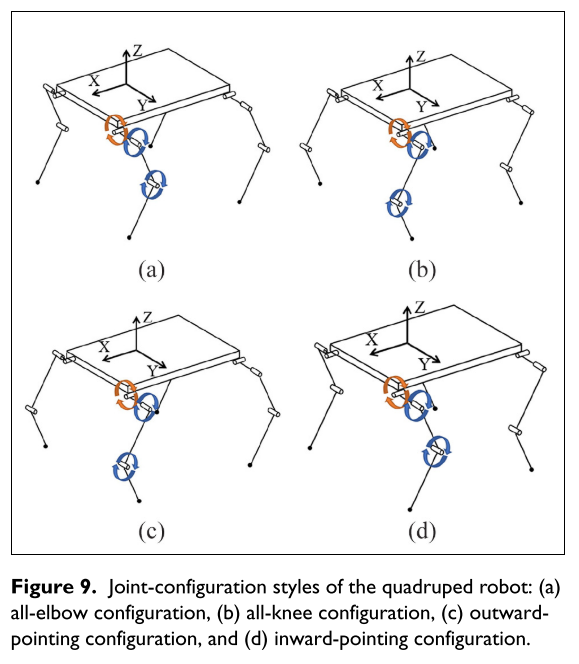
\includegraphics[width=0.5\textwidth]{joint_configurations.png}
    
    Fonte: XXX
    \label{fig:joint_configurations}
  \end{figure}

  Entre eles destacam-se o \textit{full-elbow} e o \textit{elbow-knee}. Robôs como o Spot, MIT Cheetah e Stanford Pupper utilizam a configuração \textit{full-elbow}, enquando outros como o ANYmal, StarlETH e BigDog adotam a configuração  \textit{elbow-knee}. \textbf{\textcolor{red}{\textit{Yao et al.}}} acreditam que a configuração \textit{elbow-knee} possibilita maior estabilidade, mas as características de movimento da configuração \textit{full-elbow} podem ser superiores.

  O número de juntas nas pernas, que coincide com a quantidade de DOF do robô também é um dos aspectos estudados sobre os quadrúpedes. A maioria apresenta 3 DOF por perna, o que é suficiente para que o robô consiga mover seus pés em três dimensões e realize diversos tipos de marchas. A fim de simplificar a estrutura e consequentemente o controle, alguns robôs utilizam apenas 2 DOF por perna, eliminando a junta no corpo que movimenta a perna no plano frontal. Outros buscam performances mais semelhantes ao andar de animais reais, o que aumenta a flexibilidade de movimento, justificando acrescentar uma quarta junta na perna. No entando, como já mencionado, isso aumenta a complexidade do controle e acrescenta mais atuadores ao robô, o que prejudica a eficiência.

  Essa perda de eficiência se dá porque mais atuadores significa mais consumo de energia e também mais massa. A massa do robô quadrúpede deve ser a menor possível. Quanto mais leve for o sistema, menos torque será demandado dos motores e maior sua eficiência. Além disso, a distribuição de massa do robô também deve ser considerada. A massa deve ser localizada majoritariamento no corpo, enquanto as pernas devem possuir baixa inércia. Isso as permite se mover rapidamente, sem alterar de forma significativa o centro de gravidade do robô, o que melhora a estabilidade e requer menos complexidade de controle. Possuir baixa inercia significa possuir baixa massa, porém as pernas devem ser resistentes o suficiente para suportar o peso do robô além de vários distúrbios causados pelo impacto dos pés com o chão durante a movimentação, o que pode demandar um aumento de massa. Um balanço entre massa e resistência deve ser buscado, o que reforça a necessidade de se diminuir a massa total do sistema \textbf{\textcolor{red}{[Fonte: Analysis and research of quadruped robot's legs: A comprehensive review]}}.

  \subsubsection{Atuadores}
  Robôs quadrúpedes também podem ser categorizados com base no tipo de atuadores que utilizam em suas juntas. O tipo de atuador exerce uma enorme influência na performance de movimento do robô, massa total e capacidade de \textit{payload}, assim como no sistema de controle que será utilizado das juntas. Em um estudo sobre atuadores de robôs quadrúpedes \textbf{\textcolor{red}{[Fonte: Design and driving model for the quadruped robot: An elucidating draft]}}, \textbf{\textcolor{red}{\textit{Yao et al.}}} abordam diferentes tipos de atuadores e analisam a performance de robôs quadrúpedes que os utilizam. Os três tipos principais são: hidráulicos, atuadores elásticos em série (\textit{series elastic actuators, SEA}) e motores elétricos com redução. Robôs com atuadores hidráulicos normalmente possuem mais massa e, consequentemente, maior \textit{payload} (kg), embora sua capacidade de \textit{payload} (\%) seja mais baixa. Esse tipo de atuador possui alta potência e uma performance rápida e estável. Em contrapartida, robôs com atuadores eletromagnéticos apresentam melhor movimentação e mais agilidade, sendo capazes de realizar mais tipos de marchas. Os SEAs são formados por motores elétricos e elementos elaśticos como molas, a fim de eliminar picos de torque, permitir o melhor controle do torque nas juntas e ainda aumentar seu compliance. Entre os robôs analisados, os com SEAs apresentaram maior capacidade de \textit{payload}. Os atuadores com redução são altamente utilizados com a função de aumentar o torque nas juntas, a custo de uma perda de velocidade. Eles também possui uma performance de controle de torque satisfatória. Na comparação realizada, os robôs com esse tipo de atuador apresentaram capacidade de \textit{payload} equiparada a daqueles com atuadores hidráulicos e, em geral, menor velocidade, com exceção do Cheetah 2, que está muito acima da média nesse quesito, sendo, hoje em dia, um dos quadrúpedes mais rápidos do mundo.

  Um outro tipo de atuador utilizado em robôs quadrúpedes são os servomotores: motores DC equipados com uma caixa de redução e \textit{encoder}. Esses motores são menos adaptáveis a diferentes condições do terreno, pois fornecem baixo compliance nas juntas, e possuem baixa valocidade, limitando a agilidade do robô. No entanto, produzem alto torque e permitem um preciso controle de posição. Também são mecanismo simples, leves e de baixo custo, o que os torna adequados para projetos de pesquisa e voltados para educação. O protótipo desenvolvido nesse trabalho utiliza servomotores, pois este era o recurso disponível mais facilmente.

  \subsubsection{Processamento}
  O subsistema de processamento é o responsável por processar os dados demandados por todas as funcionalidades implementadas no robô, desde as mais fundamentais como controle das juntas e de locomoção até tarefas de mais alto-nível, como inspeção ou navegação autônoma.

  Dentre os robôs que tinham seus dados de hardware reportados no review realizado por Biswal \textbf{\textcolor{red}{[Fonte: Development of quadruped walking robots: A review]}}, a maioria utiliza sistemas operacionais (SO) baseados em RT-Linux (\textit{real-time linux}) ou outros tipos de SOs de tempo real. Sistemas em tempo real são importantes, especialmente, para robôs que embarcam os controladores das juntas nos computadores de bordo, pois eles conseguem garantir o tempo execução de todo o processamento necessário para o loop de controle, o que melhora a performance e pode ser crucial para a segurança do robô e de seus operadores. Outra solução é embarcar o controle de baixo-nível em um sistema microncontrolado que se comunica com um PC para tarefas de nível mais alto, como é feito no TITAN-XIII \textbf{\textcolor{red}{[TITAN-XIII: sprawling-type quadruped robot with ability of fast and energy-efficient walking]}}.

  Tratando-se do processamento necessário pera realizar o controle de locomoção de robôs quadrúpedes, o controle das juntas, normalmente, é o que possui a frequência de operação mais alta, pois sua estabilidade é crítica para a operação do robô. O controle das juntas do ANYmal opera a 400 Hz \textbf{\textcolor{red}{[ANYmal - A Highly Mobile and Dynamic Quadrupedal Robot]}}, o do HyQ e o do TITAN-XIII a 1 kHz \textbf{\textcolor{red}{[Fontes: Design of HyQ -A hydraulically and electrically actuated quadruped robot, TITAN-XIII: sprawling-type quadruped robot with ability of fast and energy-efficient walking]}} e o do LittleDog a 500 Hz \textbf{\textcolor{red}{[Fontes: A Controller for the LittleDog Quadruped Walking on Rough Terrain]}}. Tarefas de mais alto nível são realizadas em frequências menores, pois possuem menor criticidade e maior custo computacional. Alguns robôs como o TITAN-XIII, o HyQ e o LittleDog executam essas tarefas em um computador externo, com uma conexão sem fio com o computador de bordo. Isso diminui a complexidade do sistema embarcado no robô e também sua massa total, porém aumenta o risco de erros de comunicação assim como a latência. O frequência de execução dessas tarefas também varia bastante para cada robô, afinal dependem do método de controle implementado em cada um. O LittleDog executa seu loop de mais alto-nível a 100 Hz \textbf{\textcolor{red}{[Fontes: AA Controller for the LittleDog Quadruped Walking on Rough Terrain]}}, o TITAN-XIII a 50 Hz \textbf{\textcolor{red}{[Fontes: TITAN-XIII: sprawling-type quadruped robot with ability of fast and energy-efficient walking]}} e o HyQ a 200 Hz \textbf{\textcolor{red}{[Fontes: Design of HyQ -A hydraulically and electrically actuated quadruped robot]}}.

  \subsection{Movimentação por marchas}

  \subsection{Controle de locomoção}

  \subsection{Benchmarking}

  
\end{document}
